\chapter{Background}

In this chapter, the background and fundamentals related to this thesis are covered briefly. Section \ref{stereotypes, language} provides an overview about stereotypes, their origin, their perspectives, and the role of language in the sustenance and maintenance of stereotypes. 

\section{Stereotypes, language and stereotyping} \label{stereotypes, language}
\subsection{Background}

Traditionally, there have been two kinds of cognitive processes called intuition and reason \cite{kahneman2002representativeness}. The dual process is the general label adopted wherein two cognitive operations are described with generic labels "system 1" and "system 2" \cite{kahneman2002representativeness}. System 1 describes the cognitive mode, which is intuitive and fast. System 2, on the other hand, is reflective controlled. Table \ref{tab:cognitive systems} gives an overview of the two systems. These two cognitive modes play a role in the formation of bias. Biases in cognition arise due to attribute substitution. Attribute substitution heuristics states that "when confronted with a difficult question, people often answer an easier one instead, usually
without being aware of the substitution" \cite{kahneman2002representativeness}. Simply put, the target attribute (difficult question) is substituted by a representative and available heuristic attribute (a simple question that resembles the difficult question). This substitution leads to systematic biases. These implicit/systematic biases are formed by the system - 1 due to its fast, automatic, and associative characteristic feature \cite{kahneman2002representativeness}. "System 1 generates impressions of the attributes of objects of perception and thought"\cite{kahneman2003maps}. The "impressions that are similar, especially if a label is attached, tend to cohere into categories(generalization, concepts)"\cite{fiske1998stereotyping}. Categorization leads to the generalization of group behavior, expectancies. The overgeneralized beliefs and expectancies about a category or group of people refer to stereotypes \cite{allport1954nature}\cite{fiske1998stereotyping}. 
% This cognitive representation with noisy false attributes leads to prejudice (emotion). Judging with stereotypical beliefs and prejudicial attitudes results in discrimination.

% Please add the following required packages to your document preamble:
% \usepackage{booktabs}
% \usepackage{graphicx}
\begin{table}[]
\centering
\scalebox{0.5}{
\resizebox{\columnwidth}{!}{%
\begin{tabular}{@{}ll@{}}
\toprule
System 1 (Intuitive)                  & System 2 (Reflective)              \\ \midrule
\multicolumn{1}{|l|}{Do not require working memory} & \multicolumn{1}{l|}{Requires working memory} \\ \midrule
\multicolumn{1}{|l|}{Autonomous}      & \multicolumn{1}{l|}{Controlled}    \\ \midrule
\multicolumn{1}{|l|}{Rapid, Parallel} & \multicolumn{1}{l|}{Slow, serial}  \\ \midrule
\multicolumn{1}{|l|}{Associative}     & \multicolumn{1}{l|}{Rule governed} \\ \bottomrule
\end{tabular}%
}}
\caption{Two cognitive systems }
\label{tab:cognitive systems}
\end{table}

% \pagebreak
% \begin{itemize}
%     \item Origin of bias (System -1 and system -2) ; TWO FAMILIES OF COGNITIVE OPERATIONS \cite{kahneman2002representativeness}
%     \item  How stereotypes are inevitably formed (implicit bias) ??
%     Impressions + labels ...
%     \cite{fiske1998stereotyping}
%     \item Difference between stereotype and prejudice \cite{fiske1998stereotyping}
%     \begin{itemize}
%         \item Stereotype (Cognitive) : An overgeneralized belief about a particualr group of people.This need not be negative but sometimes be accurate, like Lions have four legs. But the problem arises if the stereotype is rooted with inaccurate association formed between target from social groups (gender, ethnicity ..) and its attribute. 
%         \item Prejudice (Attitude) : "pre-judgement", typically negative attitude towards an individual or group.
%         \item Discrimination (Behaviour) : Stereotypical beliefs combined with prejudicial attitude towards social groups can drive the behavior to change which results in discrimination.\label{crashcrouse}\footnote {\url{https://www.youtube.com/watch?v=7P0iP2Zm6a4&ab_channel=CrashCourse}}
%     \end{itemize}
% \end{itemize}
\subsection{Perspectives of stereotypes}
A lot of research has been carried out on stereotypes from as early as 1927, with evolving definitions and constructs being put forth by investigators. This section defines the different perspectives of stereotypes and, finally, the perspective used in this thesis.
\\
\\
As can be seen in the table \ref{tab:stereotype_taxonomy} taken from "meaning of stereotype" in psychology
\cite{ashmore1981conceptual}, there are many perspectives concerning stereotypes. Every definition deal with a dimension of stereotype  such as "fixed, rigid", "generalization","incorrect" etc. \cite{kanahara2006review} describes that each definition belongs to combination of components ("adjectives" and "nouns") such as "superficial", "characteristic", "fixed", "image", "impression", "belief", "ethnic", "cultural" etc.  The definitions include "incorrect beliefs" \cite{katz1935racial}, "the attribution of general psychological characteristics to large human groups" \cite{watson1974psychology}, "an inaccurate, rigid, and oversimplified image of members of a social
group, especially an out group" \cite{coon1994essentials} among others. 
Among the definitions seen in the table \ref{tab:stereotype_taxonomy} and the ones stated above, the common component or dimension is "group concept (generalized)" and "beliefs."  \cite{kanahara2006review} uses these two components and posits that "stereotype is a belief about a group of individuals"  \cite{kanahara2006review}.
considering an example, "Japanese do karate"; according to the \cite{kanahara2006review}, this is a stereotype as it involves a belief (do karate) about an entire group (Japanese). "Stereotypes can be positive or negative, correct or incorrect, simple or complicated, as beliefs can be positive or negative." \cite{kanahara2006review}. According to \cite{kanahara2006review}, the beliefs about a group of people cannot be completely validated to be true.
These stereotypical beliefs, when instantiated, lead to stereotypic expectancies (stereotyping). Considering the same stereotype, "Japanese do karate," the application of this stereotype would be to judge a Japanese person by saying, "Ken must do karate because he is Japanese."
Until this point, stereotypes can be understood as generalized beliefs about a group of individuals, and stereotyping is generalized expectancies based on the belief. 

"Stereotypes are considered to be the "pictures in the head" of individuals looking out into their social worlds"\cite{macrae1996stereotypes}. Hence, one perspective is that of the generalized impressions people have in their heads. On the other hand, these generalized impressions could be shared socially among ethnic or cultural groups. This gives a socially shared perspective of stereotypes. "Stereotypes only have meaning to the extent they are socially shared"\cite{macrae1996stereotypes}. In summary, stereotypes are generalized beliefs about a group of individuals. These beliefs could be "pictures in the head," or they could be socially shared. 

In this thesis, both the perspectives, stereotypes as pictures in head and socially shared stereotypes, are considered while assessing the stereotypes encoded in the text sequences.


Considering the perspective that socially shared stereotypes only have meaning, there is a need for a medium to transmit stereotypes. Language thus plays an important role in the sustenance and maintenance of stereotypes\cite{macrae1996stereotypes}.



% \begin{itemize}
%         \item Stereotypes cannot be avoided, as they are implicitly formed as a part of the cognitive process. When these associations/ implicit bias (deviation from rationality) are overgeneralized followed by, this leads to stereotyping. Hence arises two perspectives or dimensions of stereotypes 
%             \begin{itemize}
%                 \item Stereotypes (as pictures in head / Implicit associations)
%                 \item Stereotyping (Socially shared Stereotypical associations / Overgeneralized beliefs and expectancies) 
%             \end{itemize}
%             \item Coming to this thesis, social stereotypes are being studied where the focus is mainly on examining 
%             \begin{itemize}
%                 \item Biased stereotypical associations
%                 \item Socially shared Stereotypes
%             \end{itemize}
% \end{itemize}
% \begin{itemize}
%     \item Describe two perspective, Stereotypes as pictures in head and stereotyping (shared social beliefs and expectancies)
%     \item Definitions of stereotype from other papers
%         \begin{itemize}
%             \item Stereotypes definition taxonomy \cite{ashmore1981conceptual}
%         \end{itemize}
%     \item Cognitive processes in stereotyping and intergroup behavior \cite{hamilton2015cognitive}
%     \item Stereotypes and stereotyping \cite{macrae1996stereotypes}
%     \item Prescriptive and descriptive stereotyping
%     \item Types of harms caused by bias [Kate Crawford. 2017. The Trouble with Bias. Keynote
% at NeurIPS]
% \end{itemize}
\subsection{Contribution of language}

The role of language in the maintenance of social category stereotypes is significant 
\\
\cite{burgers2020language}.
 "Social categories and Stereotypes Communication (SCSC)" 
 \cite{beukeboom2019stereotypes} mentions two broad linguistic biases, namely, linguistic labels used to refer to categorized individuals. Out of generic and specific labels all, Generic labels play a crucial role in stereotype communication\cite{burgers2020language}. Generic labels refer to a category as a whole, e.g.("women are ..."), while specific labels refer to subgroups ("Young women.."). Typically, generic labels facilitate the communication of stereotypic information when compared to specific labels\cite{burgers2020language}. 
 
 The second group of linguistic biases in stereotype communication relates to the language used in communication\cite{beukeboom2019stereotypes}. It has been shown that speakers systematically vary the language when either describing the stereotypical consistent behavior or stereotypical inconsistent behavior. The stereotypic consistent behavior is described with high essentialism  ("The rocket scientist is smart"), whereas stereotype inconsistent behavior is described as a one-time event with low essentialism and use negation to describe the one-time specific situational circumstance ("The rocket scientist is not smart")\cite{burgers2020language}.  
 \\
There is a bidirectional link between stereotype and language use, as language acts as a medium by which stereotypes are shared, and social category stereotypes, in turn, feed the medium through message recipients\cite{burgers2020language}. 
    % \begin{itemize}
    %     \item Stereotypes as collective belief systems \cite{macrae1996stereotypes}
    %     \item How language contributes to stereotype formation \cite{burgers2020language}
    %     \item How stereotypes are shared through language: a
    % review and introduction of the social categories
    % and stereotypes communication (SCSC) framework \cite{beukeboom2019stereotypes}
    % \end{itemize}
    % \pagebreak

% Please add the following required packages to your document preamble:
% \usepackage{booktabs}
% \usepackage{graphicx}
% \usepackage{lscape}
\begin{landscape}
\begin{table}[]
\centering
\resizebox{\columnwidth}{!}{%
\begin{tabular}{@{}cllcll@{}}
\toprule
\multicolumn{3}{c}{Stereotype not defined as bad, but it is a} &
  \multicolumn{3}{c}{Stereotype defined as bad generalization/category/concept; due to} \\ \midrule
\multicolumn{1}{|c|}{Generalization} &
  \multicolumn{1}{l|}{Category/concept} &
  \multicolumn{1}{l|}{Incorrectly learned} &
  \multicolumn{1}{c|}{Overgeneralized} &
  \multicolumn{1}{l|}{Factually incorrect} &
  \multicolumn{1}{l|}{Rigid} \\ \midrule
\begin{tabular}[c]{@{}c@{}}"Stereotyping may be defined as the tendency to attribute \\ generalized and simplified characteristics to group of people "\end{tabular} &
  \begin{tabular}[c]{@{}l@{}}"A stereotype is a commonly thought of \\ as a categorical response, i.e. membership  is \\ sufficient to evoke that the stimulus person\\  possess all the attributes belonging to that category"\end{tabular} &
  \begin{tabular}[c]{@{}l@{}}"Unlike other generalization ...\\  stereotypes are based on rumors, \\ anecdotes in short on evidence which \\ is insufficient to justify the generalization\end{tabular} &
  ".. a stereotype is an exaggerated belief associated with a category" &
  \begin{tabular}[c]{@{}l@{}}" A stereotype is a fixed impression, which confirms \\ very little to the fact it pretends to represent"\end{tabular} &
  "Stereotype .. the disposition to think in rigid categories" \\ \bottomrule
\end{tabular}%
}
\caption{A taxonomy of psychological meaning of the contract "stereotype" derived from Brigham's (1971) Analysis }
\label{tab:stereotype_taxonomy}
\end{table}
\end{landscape}

\section{Machine learning and deep learning}
\subsection{Machine learning pipeline}
\begin{figure}[t]
            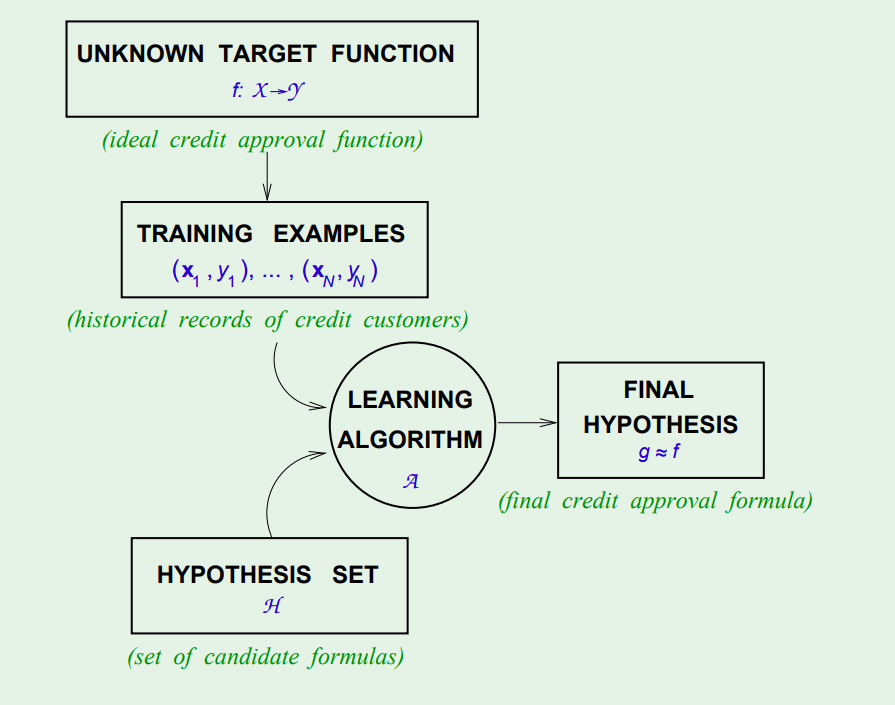
\includegraphics[width=8cm]{thesis/figures/MLpipeline.PNG}
            \centering
            \caption{The learning problem setup\cite{abu2012learning}}
            \label{fig:The learning problem setup}
        \end{figure}
Machine learning could be introduced as "learning from data" \cite{abu2012learning}. Machine learning is used when there exists a pattern that can pin it down mathematically, and last but not least, there is some data\cite{abu2012learning}. Machine learning deals with the development and analysis of a learning algorithm.  The aim of developing a learning algorithm is to use it for a specific task for a specific purpose expecting a certain quality of output\cite{abu2012learning}.  Hence, the data used to train the learner should represent the learning task in order for the learner to learn.  The goal is to learn an algorithm that generalizes across data \cite{abu2012learning}. In supervised learning (a type of learning algorithm), the learner is provided with labeled data to train on. In general, the labeled data is split into training and validation sets, and the model is trained and validated against the validation test. Finally, the model is tested on a test set that is not seen while training\cite{abu2012learning}. Defining it in more detail, the instance space is split into input space $x$ and output space $y$, and the goal is to learn a mapping from $x$ to $y$ formerly known as target function as shown in the figure \ref{fig:The learning problem setup}. In order to learn a target function g, the learning algorithm (A) is given a set of (D) training examples {x,y} belonging to input and output space\cite{abu2012learning}. At the output, the learner produces a function 'g' that is an element of hypothesis space (h) \cite{abu2012learning}. Learner (A) tries to choose a hypothesis from (h) that best fits the data (D). The result of the learning process is model (g), which tries to approximate (f)  \cite{abu2012learning}.
\subsection{Neural Networks architecture}
Conventional machine learning algorithms needed a domain expert to transform the raw input into representations or features vectors, which are then fed into the machine learning model \cite{lecun2015deep}. "Deep learning methods are representation learning methods"\cite{lecun2015deep}. "For classification tasks, higher layers of representation
amplify aspects of the input that are important for discrimination and
suppress irrelevant variations"\cite{lecun2015deep}. Figure \ref{fig:PLA} shows the perceptron learning algorithm, which is a basic neural network structure. The algorithm works in this way. Firstly, the inputs are passed along to the input layer($x_i$), next for each of these inputs, a weight ($w_i$) is being attached to either amplify or suppress the corresponding feature (which is how the neural network learn). The inputs with corresponding weights gets passed to the neuron, where the weighted sum of input values are calculated ($(\sum_{i=1}^{n}w_ix_i)$). Finally, the weighted sum is passed through an activation function to the corresponding next neuron. This forms the building block of a neural network. The neural network begins to learn by adjusting the corresponding weights attached to it.\cite{lecun2015deep} The rate of change of weight is calculated with the help of cost function or loss function. The loss function calculates the error or the loss between the output and the predicted/actual value. Based on the loss function, an error is calculated, which is backpropagated through the neural network, and the weights are thus updated based on the cost/ loss function. The algorithm that is used to update weights is called batch gradient descent\cite{lecun2015deep}. During the backpropagation, the hyperparameters, which are the tunable parameters used to control the learning process of the model, gets adjusted\cite{rumelhart1995backpropagation}.

The process of training a neural network can be broken down into forward pass and backward pass. During the forward pass, the weighted sum and the activation function are applied. Finally, an error is calculated using a loss function. During the backward pass, the loss is backpropagated to calculate the rate of change (gradients)  of weights associated with neurons. The weights are thus updated based on the gradients \cite{rumelhart1995backpropagation}\cite{lecun2015deep}. The model might overfit the training data, during training, i.e., where the training loss and validation loss have a big difference. This can be avoided by using regularization techniques where the neural network is adjusted while training to avoid this pitfall\cite{girosi1995regularization}. Regularization technique include dropout, batch normalization, etc.






\begin{figure}[t]
            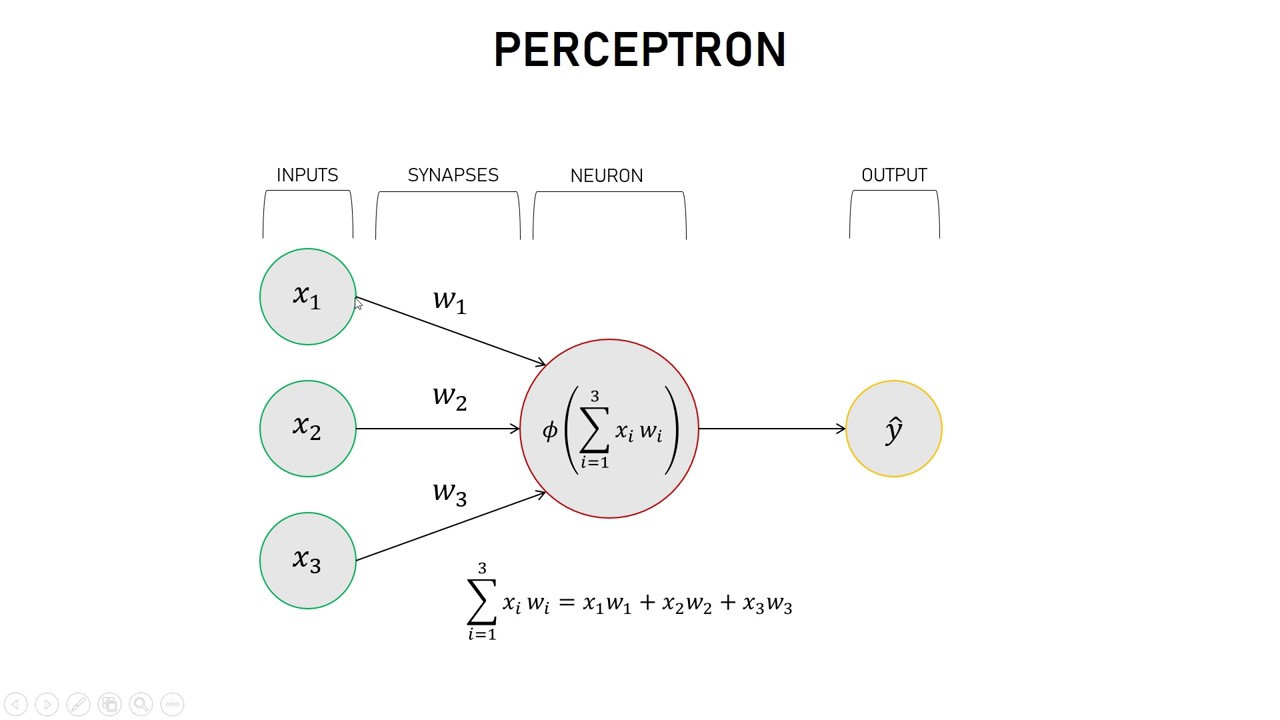
\includegraphics[width=9cm]{thesis/figures/perceptronLearningAlgo.jpg}
            \centering
            \caption{Perceptron \footnote{\url{https://www.youtube.com/watch?v=kft1AJ9WVDk&ab_channel=Polycode}}}
            \label{fig:PLA}
\end{figure}
\subsection {Recurrent Neural Networks (RNN)}
\begin{figure}[]
            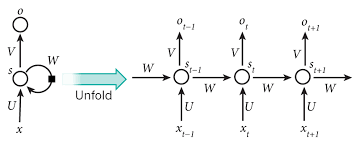
\includegraphics[width=9cm]{thesis/figures/RNN.png}
            \centering
            \caption{Recurrent neural network \footnote{\url{http://www.wildml.com/2015/09/recurrent-neural-networks-tutorial-part-1-introduction-to-rnns/}}}
            \label{fig:RNN}
\end{figure}
Recurrent neural networks short for RNN \cite{mikolov2010recurrent} are useful when dealing with sequential data. Every RNN unit contains two inputs as seen in the figure \ref{fig:RNN}, one input vector (u), one hidden state (w), and an output vector (v) at each time step. The disadvantage of vanilla RNN is that it cannot deal with long dependency. Solutions to this problem proposed with variants of RNN architecture GRU (Gated Recurrent Unit), LSTM (Long Short Term Memory Unit) \cite{mikolov2010recurrent}\footnote{\url{https://jalammar.github.io/visualizing-neural-machine-translation-mechanics-of-seq2seq-models-with-attention/}}.
\subsection{Transformer architecture}
\begin{figure}[]
         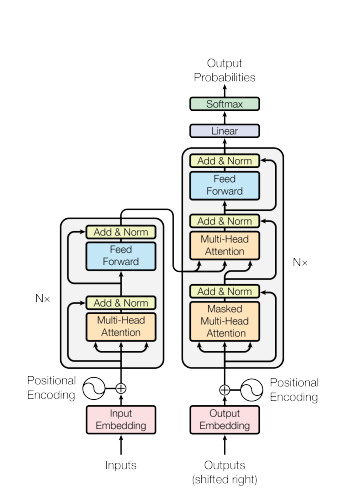
\includegraphics[width=9cm]{thesis/figures/Transformers.PNG}
            \centering
            \caption{Transformers architecture  \cite{vaswani2017attention}}
            \label{fig:Transformers}
\end{figure}

Transformers \cite{vaswani2017attention}, is a model that uses attention to boost the speed of training. The contribution of transformers, when compared to RNN, is that transformers facilitate long-range dependencies with an attention mechanism. Transformers avoid vanishing and explosion gradients as transformers do computation for the entire sequence simultaneously, and fewer training steps with no recurrence \footnote{\url{https://www.youtube.com/watch?v=OyFJWRnt_AY&ab_channel=PascalPoupart}}\cite{vaswani2017attention}.  

As can be seen in the figure \ref{fig:Transformers}, transformer consists of two blocks, namely an encoder-stack (left part of transformers) and a decoder stack (right part of the transformer). Each encoder stack takes in input word embedding as input and outputs encoded input word embedding with contextual information. The encoder stack intern consists of a feed-forward neural network, add and layer normalization, and an attention (self/multi attention head). The input is an encoded input word embedding and masked output word embedding in the decoder stack. The output of the decoder is the probability distribution over the words in the dictionary. Decoder stack consists of  an attention head (self/multi-head), add and layer normalization for regularization, encoder-decoder attention, feed-forward neural network Mainly transformers architecture was used to train on language modeling task and hence the pipeline followed by encoder and decoder stacks of transformers will be discussed .\footnote{\url{https://www.youtube.com/watch?v=OyFJWRnt_AY&ab_channel=PascalPoupart}} \cite{vaswani2017attention}

\subsubsection{Encoder-stack}
Briefly describing the encoder stack training pipeline, firstly, as shown in the figure \ref{fig:Transformers}, the inputs are fed into the encoder stack, then these inputs are converted into word embeddings. Positional encoding is added for words in sequence to provide the positional information. Multi-head attention is used to compute attention of each word in a sequence against the other words. the main idea is to treat each word as a query and find keys (other words) in the sentence based on similarity and finally compute the dot product of query and key vector to compute attention score of each word against other words. The output of multi-head attention passes through add and norm for regularization. The outputs are passed to a feed-forward layer and an add and norm for regularization. The same pipeline is repeated for the stacked encoder blocks. All the encoder receive vectors of 512, and word in each encoder flow through their own path (GPU parallelization)[5]\cite{vaswani2017attention}.

\subsubsection{Decoder-stack}
Coming to the decoder-stack, the following pipeline is followed. Firstly, as shown in the figure \ref{fig:Transformers}, word embeddings from the first iteration are given as input to the decoder-stack. It passes through positional encoding, where positional information is added. The outputs from positional encoding are passed through masked multi-head attention. The multi-head attention is masked with (-infinity) to avoid and make the self-attention to focus on previous words rather than the future words as decoder-stack of transformers are used for language modeling tasks. Then outputs pass through add and norm for regularization. The outputs now pass through multi-head attention, which taken the input from the encoder (multiple key, value pairs) and output from the masked multi-head attention of the decoder to calculate the inter attention between input and output. The outputs of the multi-head attention pass through a feed forward layer followed by add and norm followed by a linear layer with softmax activation function, which outputs probabilities over the vocabulary. The output of this is again fed as input to the decoder[5]\cite{vaswani2017attention}. 

% \section{Natural language processing and language modeling}

% \subsection{Text Representation}
% \subsubsection{Bag of words}
% A bag of words is one of the simple text representation algorithm based on word counts. The first step is to 

% \subsubsection{Term frequency and inverse document frequency}

% \subsubsection{Glove word embedding}

% \subsubsection{Fasttext word embedding}

% \subsubsection{Flair word embedding}

% \subsection{Text classification}

% \subsubsection{Multi label text classification and problem transformation}

% Data transformation is one of the methods used for dealing 
% \subsection{Text classification models}


% \subsubsection{Convolutional neural networks}
% \subsubsection{Naive bayes}
% \subsubsection{Decision trees}
% \subsubsection{SVM}

    % \begin{itemize}
    %     \item  
    %     \item Feature vectors for text 
    %         \begin{itemize}
    %             \item Bag of words
    %             \item TF-IDF
    %         \end{itemize}
    %     \item Word embeddings
    %     \item Static word embedding
    %     \item Word2vec, glove basic architecture
    % % \subsection{Text classification}    \item Text classification 
    %     \begin{itemize}
    %         \item classification types (Binary, multi class, multi label)
    %         \item LPP
    %         \item Sigmoid activation function and binary cross entropy loss function
    %         \item General text classification metrics (Accuracy, precision, recall, fmeasure)
    %         \item Multi label text classification and problem transformation 
    %     \end{itemize}
    % \end{itemize}
    % \subsection{Language modeling}
    % \subsection{Transfer learning}
    % \subsection{BERT architecture}
% \section {Evaluation metrics}    
% \section{Bias and social bias in Natural language processing}
% \begin{itemize}
%     \item A critical survey of bias in NLP \cite{blodgett2020language}
%     \item A survey on Bias in Deep NLP \cite{garrido2021survey}
% \end{itemize}